%
% einseitig.tex
%
% (c) 2024 Prof Dr Andreas Müller
%
\begin{figure}
\centering
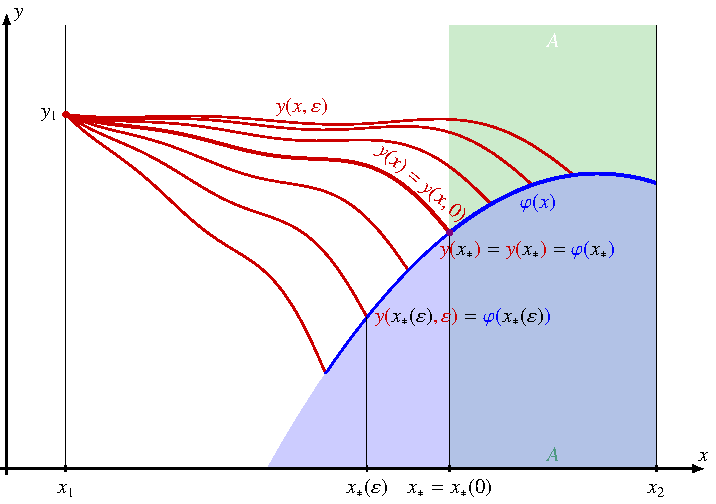
\includegraphics{chapters/050-nebenbedingungen/images/einseitig.pdf}
\caption{Herleitung der Anschlussbedingung von
Satz~\ref{buch:nebenbedingungen:einseitig:satz:anschlussbedingungen}.
Die Variation $y(x,\varepsilon)$ ist eine Lösung der
Euler-Lagrange-Differentialgleichung zwischen $x_0$ und $x_*(\varepsilon)$,
von $x_*(\varepsilon)$ and stimmt sie mit der Nebenbedingung überein:
$y(x,\varepsilon) = \varphi(x)$ für $x\ge x_*(\varepsilon)$.
\label{buch:nebenbedingungen:einseitig:fig:einseitig}}
\end{figure}
